\section{In-Field Spectral Measurements}
\label{sec:measurements}

% How to motivate our measurements?
To characterize the spectral footprint of a representative and diversely-populated area, 
we perform spectral analysis measurements in the Dallas-Fort Worth metroplex. In this section, 
we discuss the experimental setup and quantify the measurement-driven spectral activity.
 
\subsection{Wardriving Experimental Design}
\label{subsec:measurementdesign}
We employ a Linux-based 802.11 testbed, which includes a Gateworks 2358 board with Ubiquiti XR radios 
(XR9 at 900 MHz, XR2 at 2.4 GHz, XR5 at 5.2 GHz) and a DoodleLabs DL475 radio at 450 MHz. We develop 
shell scripts which utilize tcpdump to enable the testbed to work as a sniffer, recording all 802.11 
packets. However, since the Gateworks platform only updates its estimate of received signal strength 
upon the reception of a new packet (and not all relevant channel activity is 802.11 based), we employ 
a spectrum analyzer to form a notion of inter-network interference with finer granularity.  Hence, we 
also use a Rohde \& Schwarz FSH8 portable spectrum which operates from 100 KHz to 8~GHz. The portable spectrum 
analyzer is controlled by a Python script on a laptop to measure the received signal strength.


% Quantify the measurements
% Inter network interference and quantification
% Intra network interference
% Interference
Interference is a key issue in wireless network design. Despite sufficient levels of received signal, 
interference can cause channels to be unusable (e.g., due to high levels of packet loss) or unavailable 
(e.g., due to primary users in cognitive radios)~\cite{haykin2005cognitive}. 
The interference in wireless networks could be divided into two categories according to the interfering 
source: {\it (i)} intra-network interference, caused by nodes in the same network, and {\it (ii)} 
inter-network interference, caused by nodes or devices outside of the network. 

We define an activity level to quantify the spectrum utilization. The activity level is the percentage 
of time which the interfering signal could impact an active wireless link. In practice, we use the sensing 
samples ($S_\theta$) above an interference threshold ($\theta$) over the total samples ($S$) in a time 
unit as the activity level ($A$) of inter-network interference:
\begin{equation}
\label{eq:actdef}
A=\frac{S_\theta}{S_a}
\end{equation}



% Clearify
To the best of our knowledge, there is no readily available mobile, multiband antenna from 450 MHz to 5.2 
GHz on the market. Thus, we use a 700-MHz mobile antenna to perform spectral analysis measurements. We then 
normalize the mobile antenna performance across bands with indoor experimentation. To do so, we use a 
Universal Software Radio Peripheral (USRP) N210 to generate signals at 450 MHz, 800 MHz, and 2.4 GHz. We 
feed the USRP signals directly to a spectrum analyzer and adjust the configuration of USRP to make the 
received signal strength in the receiver side the same as the 5.2 GHz signal from Gateworks 2358 with 
a XR5 radio. 
Then, we connect the signal source to a fixed multiband antenna (QT 400 Quad Ridge Horn Antenna) and 
measure the received signal at a fixed distance with the 700-MHz antenna. We compare the received 
signals from the antennas designed for each band with known gains to obtain the antenna loss for 
each band. We further adjust the received signal strength collected via the 700-MHz mobile antenna 
according to the normalization data set.

  \begin{figure}
  %\vspace{-0.0in}
  \centering
  \includegraphics[width=74mm]{figures/equipment}
  \vspace{-0.1in}
  \caption{Multiband Measurement Platform}
  \label{fig:equipment}
  \vspace{-0.3in}
  \end{figure}
  
% Duplicate measurement in WiFi
Our experimental platform is shown in Fig.~\ref{fig:equipment}. The mobile spectrum analyzer records 32 samples 
per second on each band under test with appropriate time stamps. The Gateworks sniffer platform also records all 
the received WiFi packets according to their time stamps. The duplicate samples in the WiFi bands reported by the spectrum analyzer 
and Gateworks are removed according to overlapping time stamps to calculate the activity level in the WiFi 
bands. The activity level of white space bands is calculated solely based upon the spectrum analyzer measurements 
since it is assumed that device operating in the white space bands is not yet 802.11 compliant.

Fig.~\ref{fig:drivemap} depicts a map of the FCC-approved white space channels with markers where we performed 
measurements in North Texas. To be representative of a broad range of community types, we consider populations of 
approximately 25 times one another according to the 2010 U.S. Census: Millsap (500), Weatherford (25K), and Dallas 
(1.25 M). We have collected measurements at multiple types of locations in Dallas, including a downtown area,
a residential area, and a university campus. In Weatherford and Millsap, we monitor wireless activities in three 
locations for 45 continuous minutes on a weekday in downtown, residential, and non-residential areas. Then, we 
post-process the data to calculate the activity level of each band at each location. First, we parse the SNR from 
the data logs via Perl scripts. Second, we merge the data from the two platforms according to their respective 
time stamps and calculate the activity level of each band across these locations. The activity level is then 
included in our framework as input parameter. 

\subsection{Highway Speeds to Fixed Locations} 
\label{subsec:measurementresult}
As an initial experiment, we perform a drive test from Dallas to Weatherford with cruise control set to 60 MPH while 
on the highway. The result of the in-field spectrum drive test is shown in Fig.~\ref{fig:drivetest} according to 
the location of the measurement. The measured activity via RSSI of 450 MHz is high in downtown Dallas and 
Fort Worth but has less spectral activity in the urban and rural area between these city centers. The low activity 
detected in the WiFi bands is due to the distance from the highway being typically larger than the propagation range 
of predominantly indoor wireless routers.

Our initial spectral analysis measurements agree with the the FCC restrictions (shown in Fig.~\ref{fig:drivemap}), 
greater spectrum utility by TV bands induce less spectral availability.
The drive test also shows that the spectrum 
utilization is roughly proportional to the population density in Fig.~\ref{fig:drivetest}. We use the measurements 
collected at fixed locations as marked on the map for the activity level calculation. 

\begin{figure}
%\vspace{-0.0in}
\centering
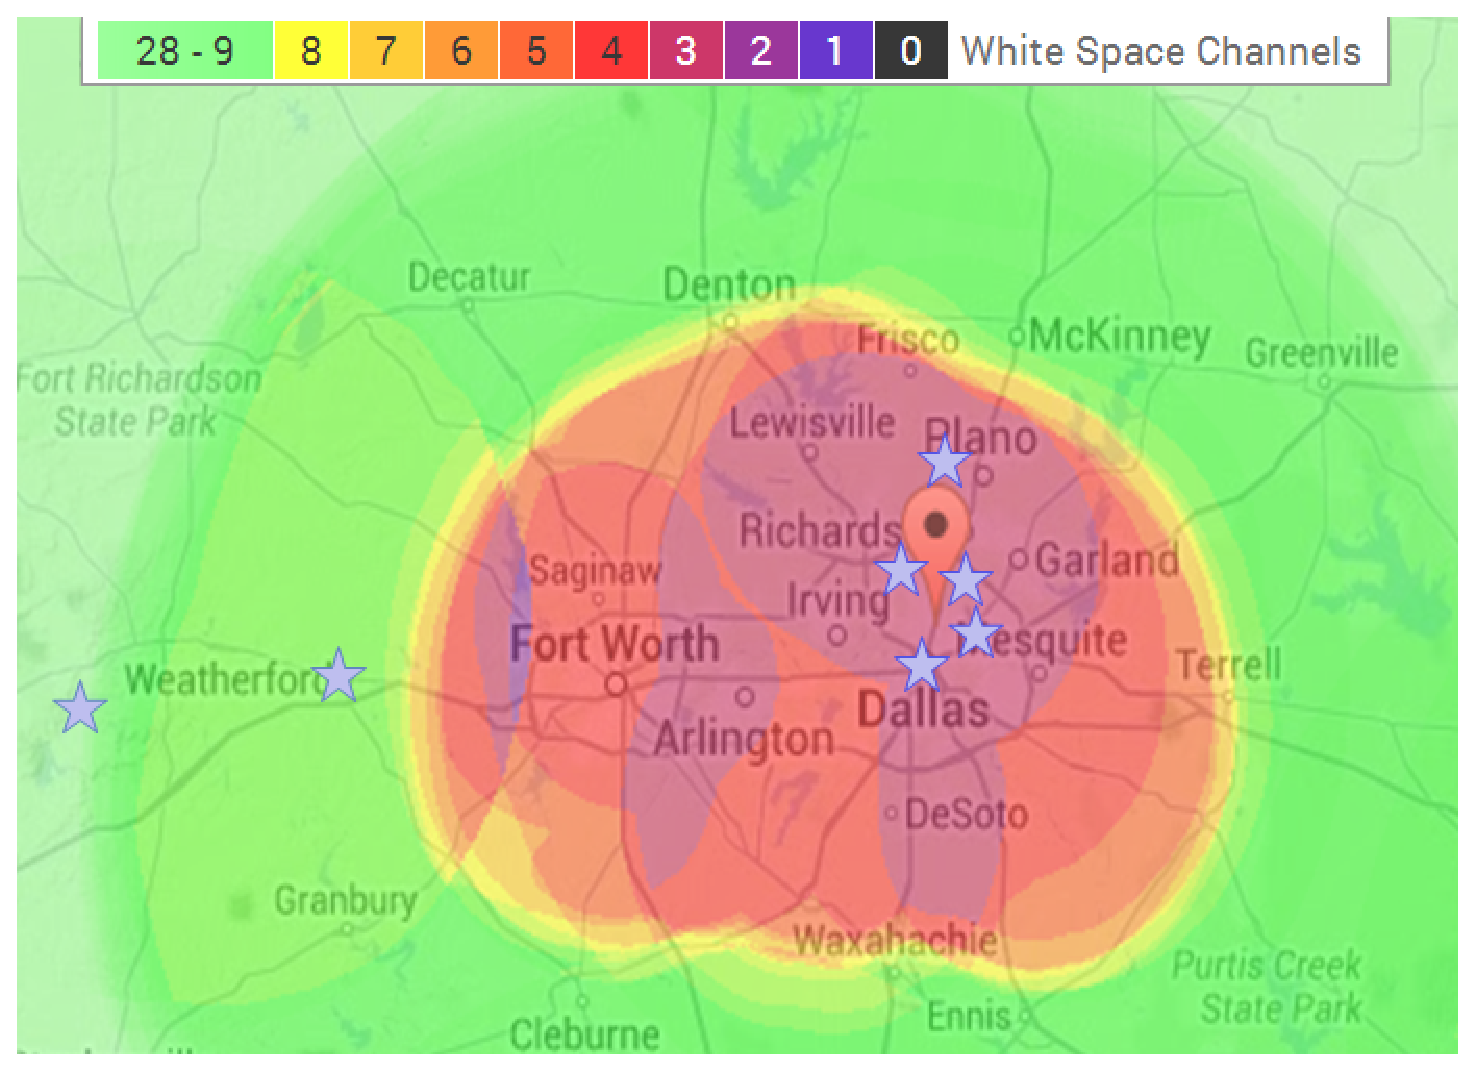
\includegraphics[width=74mm]{figures/drivemap}
\vspace{-0.1in}
\caption{White Space Channels in DFW Metropolitan and Surrounding Areas.}                                                                 
\label{fig:drivemap}
\vspace{-0.1in}
\end{figure}
   
\begin{figure}
%\vspace{-0.0in}
\centering
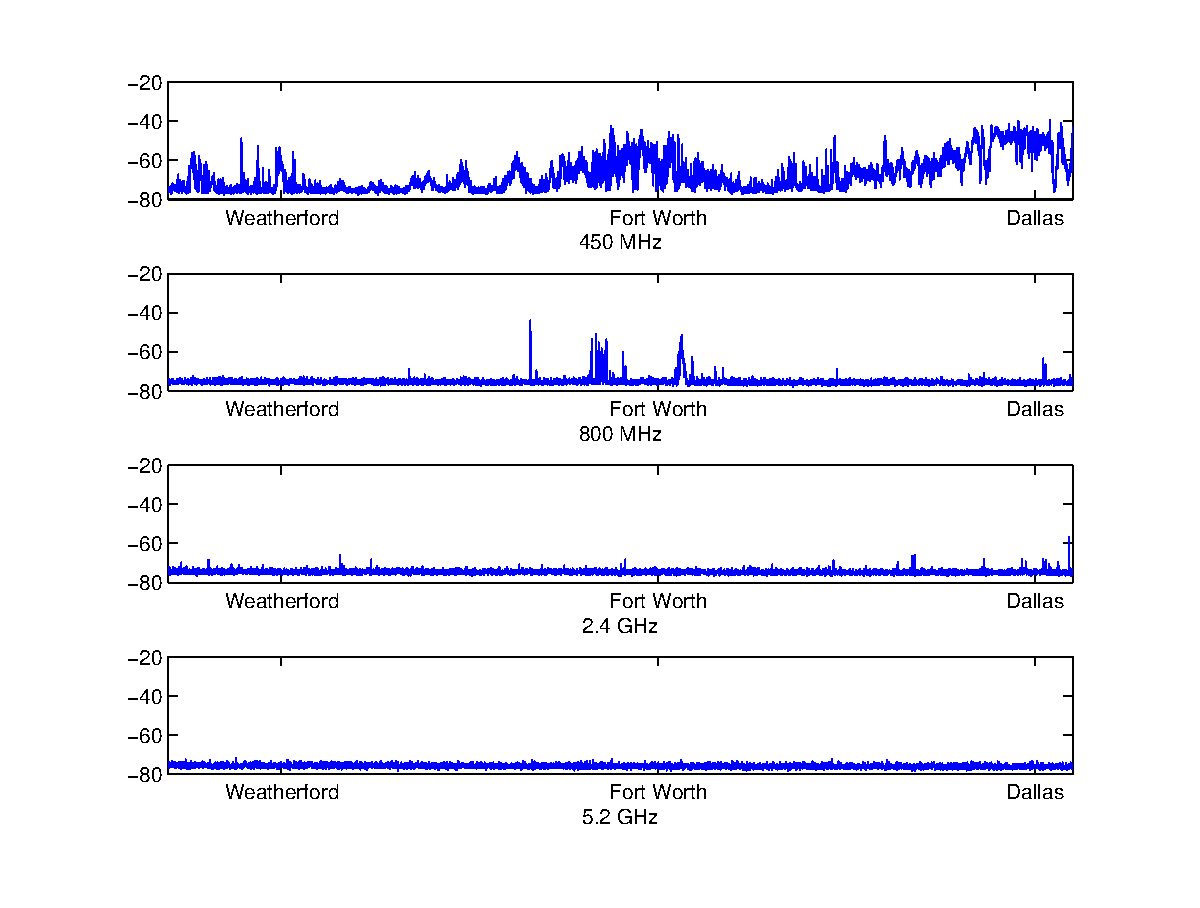
\includegraphics[width=84mm]{figures/drivetest}
\vspace{-0.3in}
\caption{Spectrum Activity in DFW Metropolitan and Surrounding Areas.}                                                                 
\label{fig:drivetest}
\vspace{-0.2in}
\end{figure}




% Here

The activity level calculated with our measurements are shown in Table~\ref{tab:activitymeasurement}. Dallas, the 
city with the greatest population in North Texas, has the highest activity level in most of the measured bands, 
especially at 450 MHz. The Dallas urban measurements are taken from the SMU campus, two neighborhoods, and a 
densely-populated suburb (Plano). Our measurements indicate that 2.4 GHz has a higher activity level in the aforementioned urban areas 
than the measured downtown area. Most schools and their neighborhoods are covered by WiFi, which contributes to the 
high activity level at 2.4 GHz and 5.2 GHz. In Weatherford, all the bands have lower activity levels than in Dallas. 
A peculiarity in the measurements can be seen by the sparse area in Weatherford having more activity than the other 
regions for 450 MHz. This can be explained due to the measurement location being on the East side of Weatherford (closer 
to Fort Worth, which has a population of approximately 750k). Millsap is a typical sparse rural area with approximately 
500 total residents. The activity levels across all the bands are lower than in Dallas and Weatherford. In the 450 MHz 
band, the activity level decreases much faster than in other bands in Dallas and Weatherford. 

\begin{table*}
\centering % centering table 
\begin{tabular}{|l|c|c|c|c|c|c|c|c|c|c|c|} % creating 12 columns 
\hline %\hline % inserting double-line 
Bands     & \multicolumn{3}{c|}{Dallas} & \multicolumn{3}{c|}{Weatherford} & \multicolumn{3}{c|}{Millsap} \\% [0.5ex]
\hline % inserts single-line 
% Entering 1st row 
Area Type & Downtown & Residential & Suburban & Downtown &  Residential & Sparse & Downtown & Residential & Sparse \\ % [0.5ex]
\hline % inserts single-line 
450 MHz &24.37	&25.83  &23.77	&6.05 &12.50  &14.03 & 7.00 & 0.07 & 0.02 \\      
\hline % inserts single-line                                                                                                       
800 MHz &4.40 	&16.49  &4.77	&5.22&5.07 &4.43  & 3.87 & 4.20 & 3.60 \\      
\hline % inserts single-line                                                                                                      
2.4 GHz &15.87 	&34.95  &2.60	&2.03&2.03 &2.77  & 2.07 & 1.60 & 0.80 \\      
\hline % inserts single-line                                                                                                     
5.2 GHz &19.70	&35.46  &1.53	&1.93&1.93 &1.33  & 1.27 & 2.07 & 2.10 \\      
\hline % inserts single-line 
\end{tabular}    
\caption{Activity Level in Multiple Locations} % title name of the table 
\label{tab:activitymeasurement}    
\vspace{-0.3in}
\end{table*}    


% Need a summary
Our measurements verify the channel occupancy variation in the DFW metroplex and quantify the occupancy
through a measurement-based activity level. The results show the spectrum bands have greater occupancy in
densely-populated areas. The measurements 
methods and resulting quantification provides the way to 
understand a typical deployment environment. We apply these 
measurements to our MAPE framework in Section.~\ref{sec:winmee} and BPS algorithms in Section.~\ref{sec:whitemesh} to 
further design access tier network deployments and backhaul tier multiband channel assignment, respectively.
